\section{Introduction}
Segmentation is often a first step when modeling trajectories of a human teleoperator executing a multistep task.
This approach has been applied in robot skill-learning \cite{calinon2010learning, kruger2010learning, konidaris2011robot}, generalization to novel initial conditions in Learning from Demonstrations \cite{Niekum2015}, and operator skill classification \cite{Reiley2009}.
Segmentation models fall into three broad categories: (1) dictionary-based, (2) label-based, and (3) unsupervised.
Dictionary-based approaches set a pre-defined vocabulary of primitives \emph{a priori} and decompose new trajectories in terms of the primitives.
Label-based approaches require annotation of examples segments, and learn a segmentation policy from examples.
Unsupervised methods assume some structure to the data, e.g., local linearity, and fit trajectories to this model grouping together locally similar points.
Unsupervised techniques can avoid time consuming labeling or dependence on a pre-defined set of primitives.

Increasingly, fixed camera video recordings accompany kinematic recordings of human teleoperation in a variety of datasets [cite].
Video can provide important information about the state of the environment and the relative orientation of the robot and other objects.
This information is crucial for segmentation that does not overfit to the robot's exact position and learns higher level task properties (i.e., the robot needs to contact an object).
While label- and dictionary-based approaches have been applied to segment multi-modal demonstrations\cite{DBLP:dblp_conf/wacv/LeaHV15,zappella2013surgical}, existing unsupervised approaches rely on hand tuned features (Krishnan et al. [cite]) or poses for all objects in the workspace via AR markers (Neikum et al. [cite]).
Leveraging raw visual data, i.e., pixels, for unsupervised segmentation is challenging due to the dimensionality and the featurization problem.

\begin{figure}[ht]
\centering
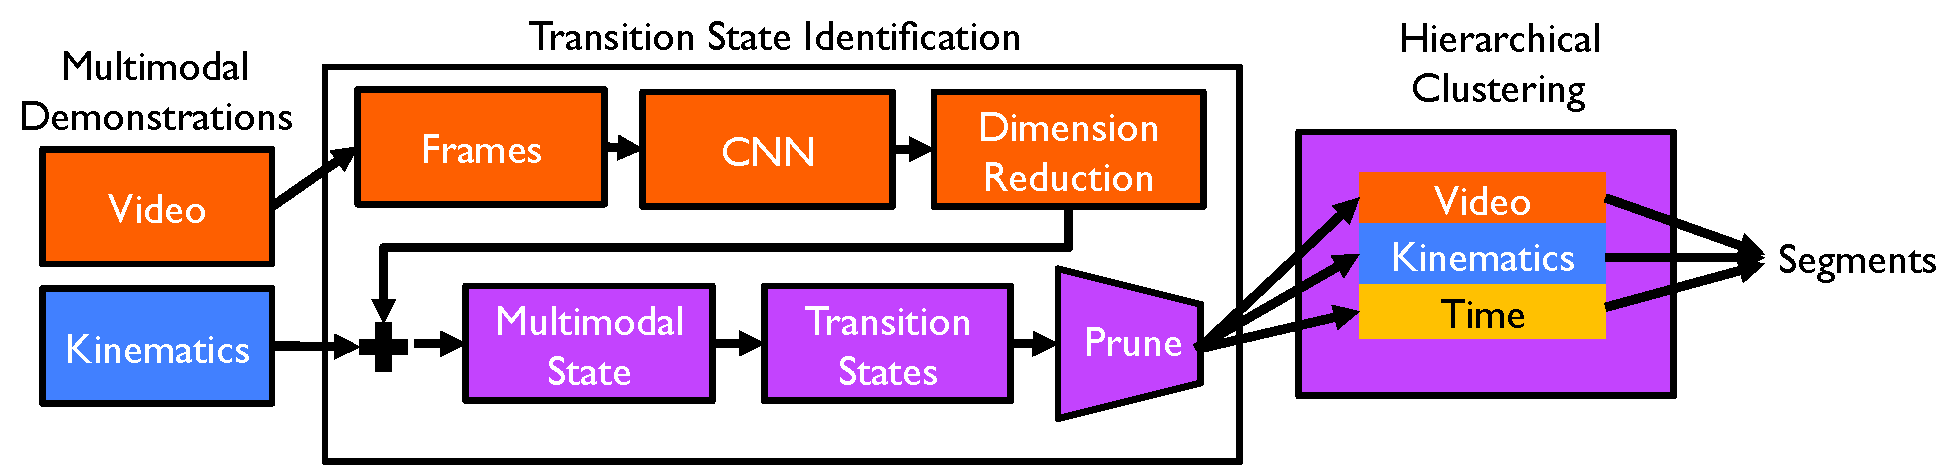
\includegraphics[width=\columnwidth]{figures/architecture.pdf}
\caption{\todo{name} architecture. We use a pre-trained CNN to featurize raw video data for use in segmentation. After featurization, we combine the data with kinematic data and apply a Transition State Clustering algorithm to identify segments. \label{fig:arch}}
\vspace{-1em}
\end{figure}

An application of particular interest is robotic surgery.
There are large and growing datasets of teleoperated surgical tasks with kinematic and camera recordings.
These recordings can facilitate automation via finite state machines, but a first step is segmentation.
In our prior work (Krishnan et al. [cite]), recognizing a number of surgery specific challenges such as temporal inconsistency and looping e.g., where a surgeon may attempt insertion 2-3 times, we proposed a non-parametric Bayesian model called Transition State Clustering (TSC).
Essentially, the model identifies states that mark linear dynamical regime transitions and clusters these states across demonstrations considering both spatial and temporal similarity.
Our results on real and synthetic data suggests this model is more robust to the demonstration inconsistencies prevalent in surgical tasks, even when these tasks were executed in a consistent environment (i.e., identical tissue phantoms). 

In this paper, we propose a \todo{name} algorithm that applies unsupervised segmentation to surgical demonstrations consisting of kinematic trajectories and video data.
To address the featurization problem in video, we leverage the growing maturity of Convolution Neural Networks (CNNs) in computer vision.
There are a number of architectures  (e.g., AlexNet [cite]) that are trained on immensely large datasets of nature images, and these pre-trained models can be applied to featurize video.
However, using a CNN as a featurizer is only part of the solution.
We design a variant of the TSC method to jointly consider both kinematic and high-dimensional featurized video data.
We illustrate the architecture in Figure \ref{fig:arch}.

In this application, pre-trained neural networks give us a convenient and transferable featurization.
We can leverage large datasets without having to do the training ourselves.
These results are complementary to the Bayesian model described in our prior work.
We model demonstrations as a time-varying stochastic process, with a discrete set of switching points.
At each time $t$, there is a hidden latent state that generates both the kinematics and video data.
Our goal is to define a segmentation w.r.t to that hidden state.
The algorithm that we propose in this paper is one approach to fit parameters to this model.

\todo{add about CCA if it pans out, add about fine tuning}

In summary, our contributions are as follows:
\begin{enumerate}
\item We propose an algorithm to segment demonstrations from kinematic and raw video data via a pre-trained CNN.
\item We describe a generative model to integrate the two types of data with dimensionality reduction.
\item We provide a comprehensive evaluation of parameters and model choice when using pre-trained CNNs for use with robotic demonstrations.
\item \todo{results suggest...}
\end{enumerate}

